\section{Introduction and smoothness coordinate}\label{sec:foundation}
Quadratic finite-difference penalized least squares (PLS) has a long history in Whittaker--Henderson smoothing \citep{whittaker1923,guerrero2007}. The penalty $\lambda$ is mathematically convenient, but the same numerical value need not express the same smoothness for different difference orders or sample lengths. Guerrero's trace-based smoothing measure \citep{guerrero2008} and its use with CV, GCV, AICc and BIC \citep{cortes2017} are established precedents. We do not claim to invent the smoother or its tuning criteria; instead, we investigate the \emph{computational cost of an interpretable bounded coordinate and the reuse of its mapping across many evaluations}.

For $y\in\R^n$, difference order $1\le d<n$, and fixed mean of the penalized differences $\mu$, let $D_d\in\R^{(n-d)\times n}$ denote forward differences and define
\begin{equation}\label{eq:pls}
\widehat\tau_{\lambda,\mu}
=\arg\min_\tau\{\|y-\tau\|_2^2+
\lambda\|D_d\tau-\mu\mathbf1\|_2^2\}.
\end{equation}
Put $r=n-d$, $Q_d=D_d^\top D_d$, and $H_\lambda=(I+\lambda Q_d)^{-1}$. A polynomial particular solution is $p_{\mu,t}=\mu\binom{t-1}{d}$, and $\widehat\tau=p_\mu+H_\lambda(y-p_\mu)$. The penalty has a $d$-dimensional polynomial nullspace, so $\tr(H_\lambda)\to d$ as $\lambda\to\infty$.

Write $\delta_1,\ldots,\delta_r>0$ for the positive eigenvalues of $Q_d$. We use the normalized smoothness index
\begin{equation}\label{eq:S}
S_d(\lambda)=\frac{n-\tr(H_\lambda)}{n-d}
=\frac1r\sum_{j=1}^{r}\frac{\lambda\delta_j}{1+\lambda\delta_j}.
\end{equation}
Each $\delta_j>0$ implies $S_d'(\lambda)=r^{-1}\sum_j\delta_j/(1+\lambda\delta_j)^2>0$, hence $S_d$ is continuous, strictly increasing, and maps $[0,\infty]$ onto $[0,1]$. Every interior $s$ has a unique penalty $\Lambda_{n,d}(s)$. The map depends only on $(n,d)$, \emph{not} on observations or the fixed reference mean $\mu$. Therefore it can be cached across different series, criteria and $\mu$ values. The denominator $n-d$ normalizes an established trace-based index; it is not a new statistical model.

\subsection{Shift-free full spectral reconstruction}
Let $D_d=U\diag(\sigma)V^\top$ be a reduced SVD over the $r$ positive singular modes and write $w_j=\lambda\sigma_j^2/(1+\lambda\sigma_j^2)$. A numerically useful identity is
\begin{equation}\label{eq:shiftfree}
\begin{aligned}
\widehat\tau_{\lambda,\mu}
=y-V\bigl[&w\odot(V^\top y)\\
&-\mu(w\oslash\sigma)\odot(U^\top\mathbf1)\bigr],
\end{aligned}
\end{equation}
where multiplication and division are componentwise. It avoids forming the potentially enormous polynomial $p_\mu$ at high $d$ and costs $O(nr)$ for a complete curve once the SVD is available. A separate high-precision companion manuscript evaluates its numerical accuracy. Here we study \emph{runtime costs} without treating a numerically invalid fast method as a winner.

The exact endpoints are interpolation at $s=0$ and the polynomial-constrained limit at $s=1$, which is evaluated analytically rather than factorizing a matrix at $\lambda=\infty$. Figure~\ref{fig:coordinate} illustrates why a user benefits from a common unit-interval smoothness coordinate even though the corresponding penalty scales vary with $d$.

\begin{figure}[t]\centering
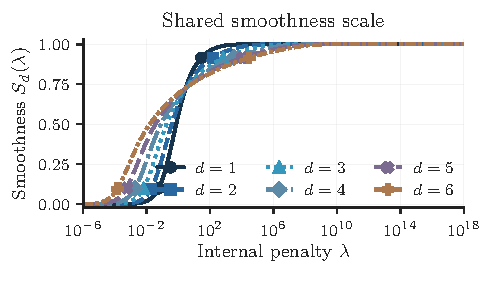
\includegraphics[width=\columnwidth]{figures/coordinate_map.pdf}
\caption{Smoothness versus penalty for $n=48$, orders $d=1,\ldots,6$. The sixth-order line illustrates the mathematical mapping, not a completed Windows timing benchmark for $d=6$.}
\label{fig:coordinate}
\end{figure}

\subsection{Research questions}
A single fitted curve, one criterion score, a complete grid search, and $R$ independent searches are different workloads. We distinguish: setup costs; full fitted-trend reconstruction; trace and leverage evaluation for CV/GCV/AICc/BIC/MLE; one-point evaluation; matched 17-point grids; locally optimized continuous searches; and repeated-series reuse. Spectral preprocessing may be expensive for one query yet efficient when amortized. The question is not whether $s$ magically lowers the cost of optimizing $\lambda$, but whether the \emph{same exact set} $\Lambda_{n,d}(s_j)$ can be calculated once, reused, and exposed to users as interpretable $s_j\in[0,1]$.
